\documentclass{beamer}
\usepackage[english]{babel}
\usepackage{color}
\usepackage{hyperref}
\usepackage{graphicx}
\usepackage[utf8x]{inputenc}
\usepackage[version=3]{mhchem}
\usepackage{amsmath}
\usepackage{amssymb}
\usepackage{amsfonts}
\usepackage{amsopn}
\usepackage{braket}
\usepackage{bbm}
\usepackage{dsfont}
\usepackage{kpfonts}
% \usepackage{mathabx}

\parindent=0cm


% Various new commands that ease typesetting math even further
% \newcommand{\assign}{\ensuremath{\coloneq}}
% \newcommand{\rassign}{\ensuremath{\eqcolon}}
\newcommand{\assign}{\ensuremath{:=}}
\newcommand{\rassign}{\ensuremath{=:}}

\newcommand{\of}[1]{\ensuremath{\left( #1 \right)}}
\newcommand{\ofs}[1]{\ensuremath{\left( #1 \right)}}

\newcommand{\norm}[1]{\ensuremath{\| #1 \|}}

\newcommand{\tmop}[1]{\ensuremath{\operatorname{#1}}}

\newcommand{\id}{\ensuremath{\mathds{1}}}
% \newcommand{\id}{\ensuremath{I}}


\newcommand{\conj}[1]{\ensuremath{\overline{#1}}}

\newcommand{\T}{\ensuremath{{}^{\textnormal{T}}}}
\newcommand{\herm}{\ensuremath{{}^{\textnormal{H}}}}

\newcommand{\ft}[1]{\ensuremath{\mathcal{F}\left(#1\right)}}
\newcommand{\ift}[1]{\ensuremath{\mathcal{F}^{-1}\left(#1\right)}}

\newcommand{\fft}[1]{\ensuremath{\mathtt{FFT}\left(#1\right)}}
\newcommand{\ifft}[1]{\ensuremath{\mathtt{IFFT}\left(#1\right)}}

\newcommand{\dotp}[2]{\ensuremath{\langle #1 , #2 \rangle}}

\newcommand{\bigO}[1]{\ensuremath{\mathcal{O}\left( #1 \right)}}

\newcommand{\mat}[1]{\ensuremath{\mathbf{#1}}}

% multi-indices
\newcommand{\mindex}[1]{\ensuremath{\underline{#1}}}

\newcommand{\laplace}{\ensuremath{\operatorname{\Delta}}}

% EOF


\mode<presentation>
{
  \usetheme{Montpellier}
  \setbeamercovered{transparent}
}

\synctex=1
\parindent 0pt

\title[Numerical Steepest Descent for Hagedorn Wavepackets]
      {Application of Numerical Steepest Descent \\
       for Overlap Integrals \\
       of Semiclassical Wavepackets}
\author[]{Raoul Bourquin}

\date{Disentis 2014}

\beamertemplatenavigationsymbolsempty
% -----------------------------------------------------------------------------------------
\begin{document}

\begin{frame}
  \titlepage
\end{frame}

\begin{frame}{Outline}
  \tableofcontents
\end{frame}


\section{Motivation}

\begin{frame}{Motivation}
  \begin{itemize}
    \item Simulation of heavy \ce{Hg2}
    \begin{itemize}
      \item Initial value $\ket{\Psi_0}$
      \item Time-propagated value $\ket{\Psi_t}$
    \end{itemize}
  \end{itemize}
  \begin{figure}
    \centering
    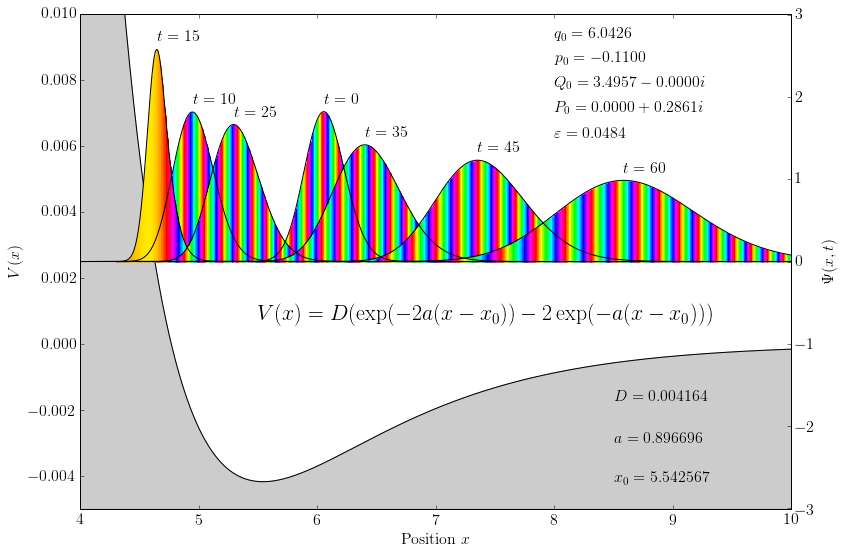
\includegraphics[width=0.7\linewidth]{./fig/hg_morse_wps.png}
  \end{figure}
\end{frame}


\begin{frame}{Motivation}
  \begin{itemize}
    \item Compute autocorrelation $|A(t)|$
  \end{itemize}
  \vspace{0.2cm}
  \begin{equation*}
    A(t) \assign \Braket{\Psi_0 | \Psi_t}
         = \idotsint_{\mathbb{R}^D} \conj{\Psi_0(\vec{x})} \Psi_t(\vec{x}) \di{\vec{x}}
  \end{equation*}
  \begin{figure}
    \centering
    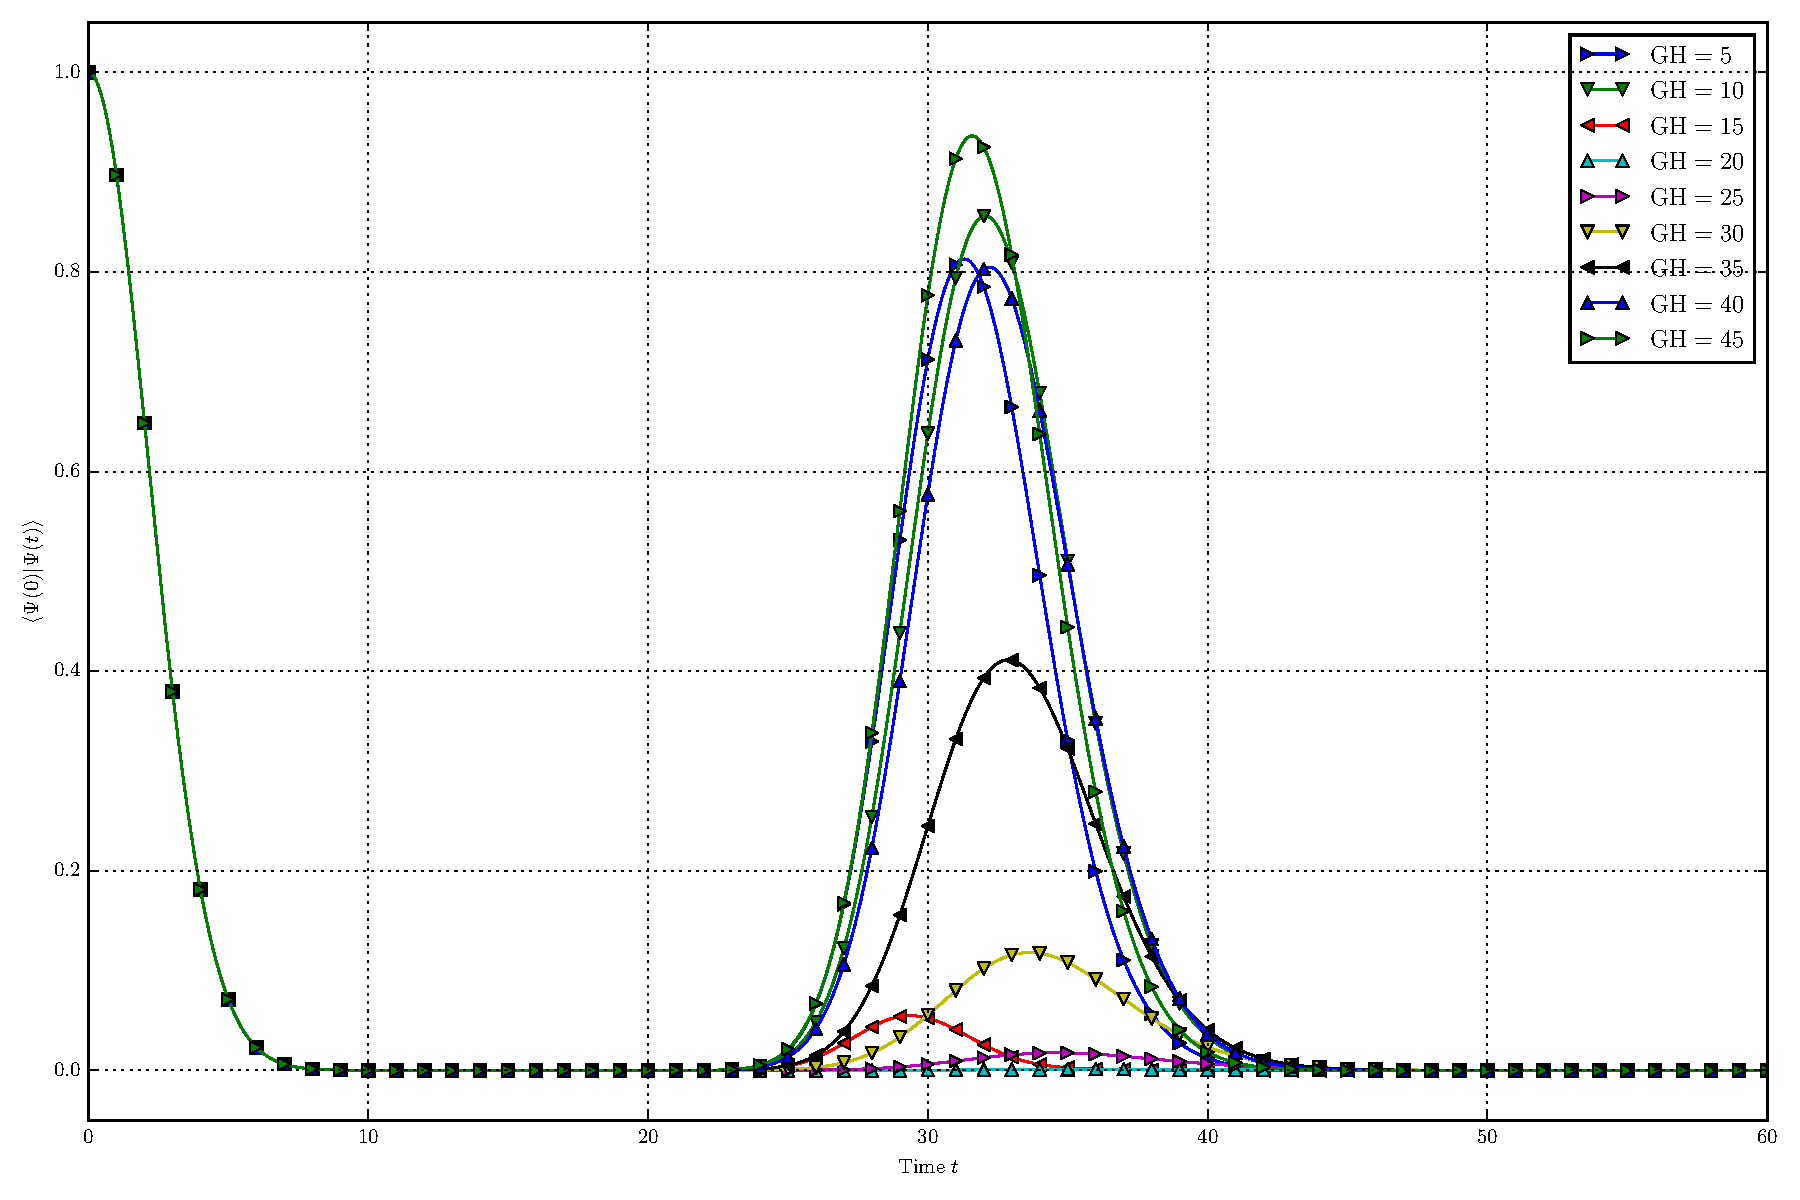
\includegraphics[width=0.7\linewidth]{./fig/ac_mercurial_morse.pdf}
  \end{figure}
\end{frame}


\section{Highly Oscillatory Integrals}
\subsubsection{Introductionary Example}

% Example with straight paths int_a^b dx


\begin{frame}{Highly Oscillatory Integrals}{Examples}
  \begin{equation}
    x
  \end{equation}
\end{frame}



\subsubsection{More complicated Example}

% Single stationary point


\section{The Steepest Descent Method}

% Handle boundaries
% Handle stationary points
% Show theorems about exact decomposition (maybe?)



\section{Hagedorn Wavepackets}
\subsection{Definition}


\begin{frame}{Semiclassical Wavepackets}
  \begin{figure}
    \centering
    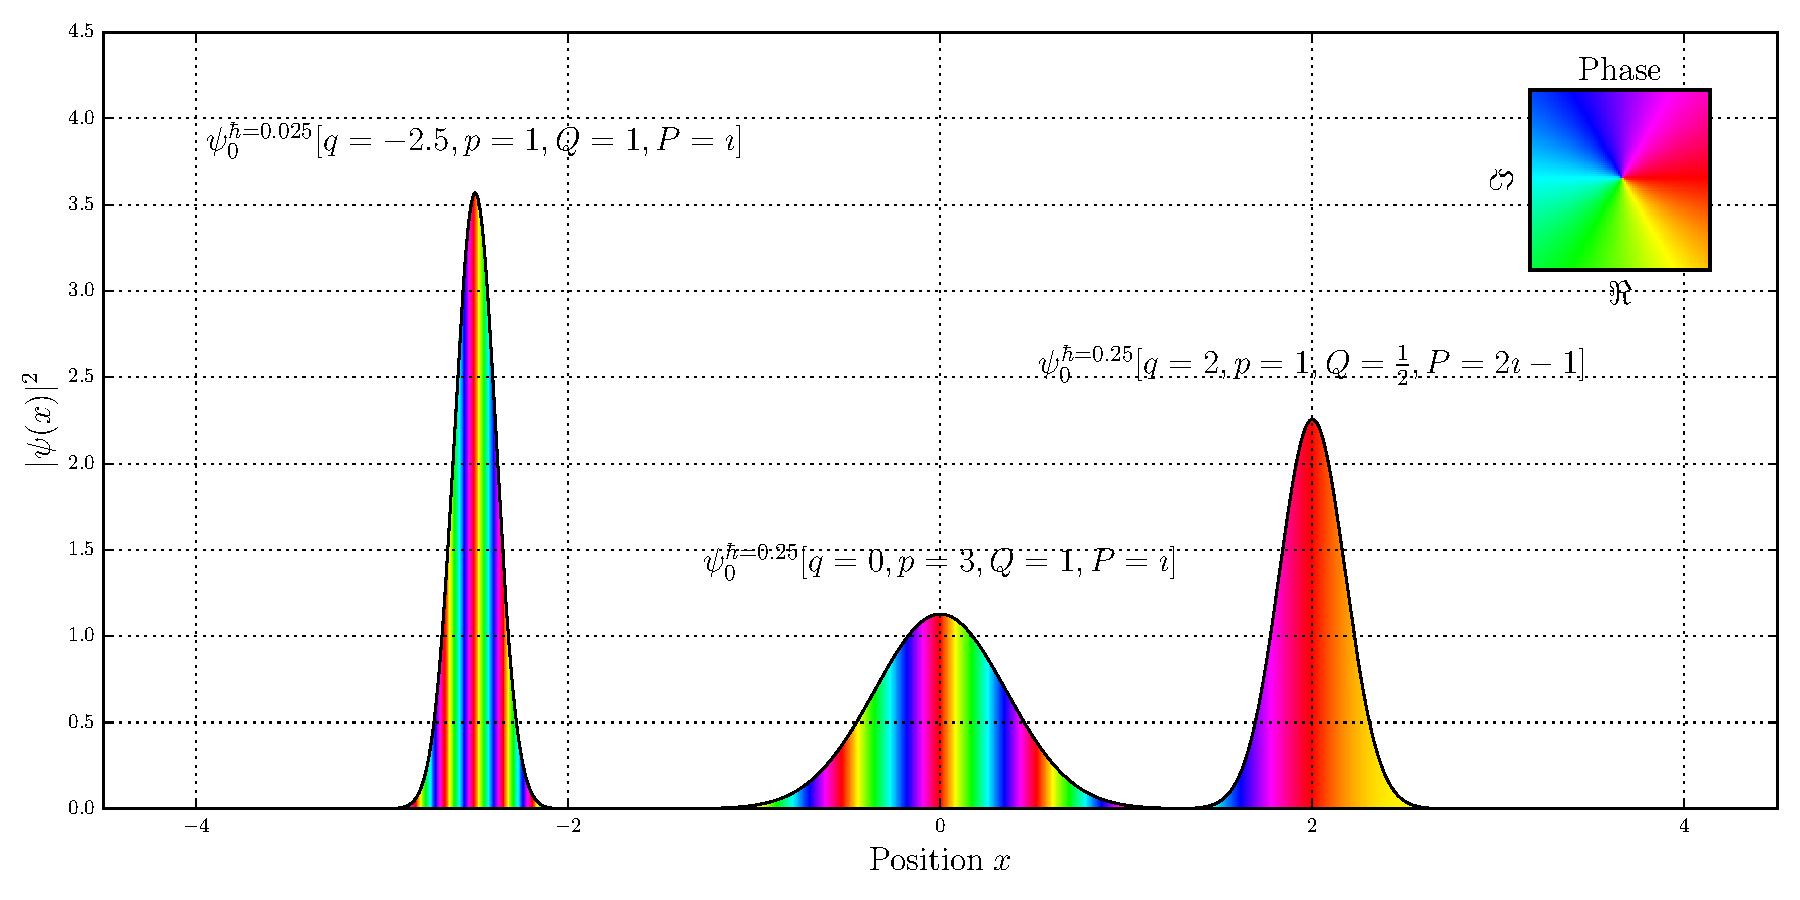
\includegraphics[width=\linewidth]{./fig/wavepackets.pdf}
  \end{figure}
\end{frame}

\begin{frame}{Semiclassical Wavepackets}
  \begin{figure}
    \centering
    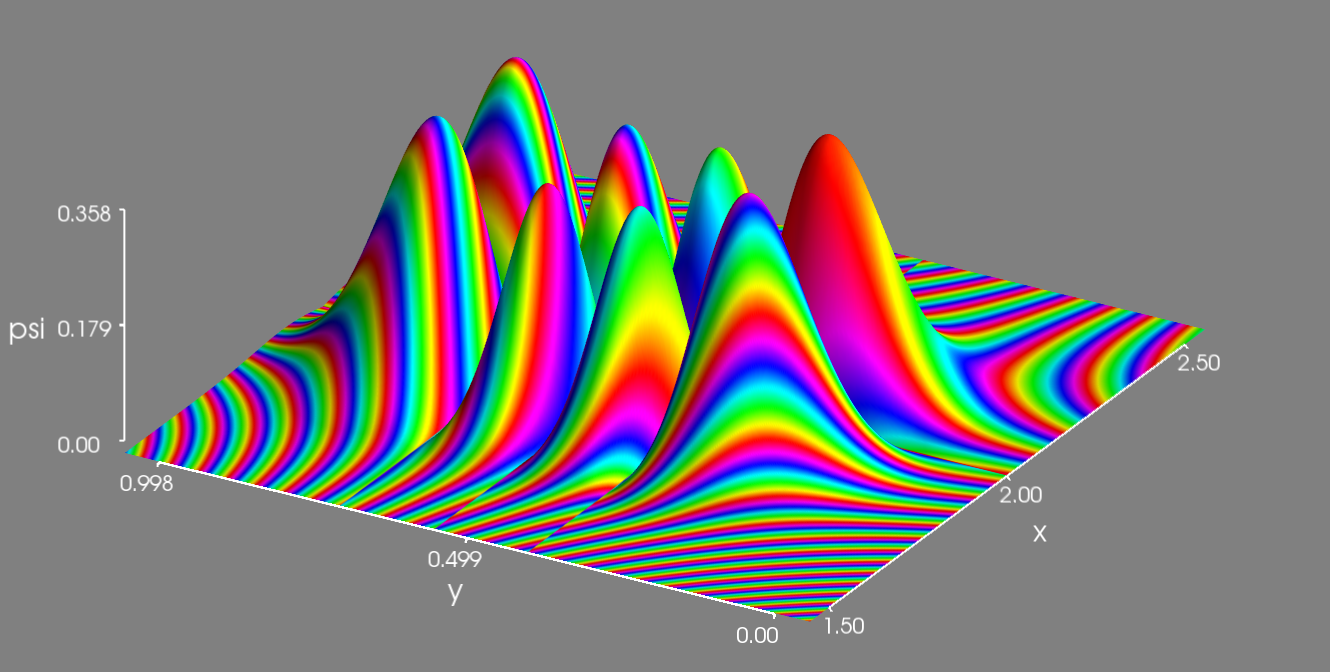
\includegraphics[width=\linewidth]{./fig/wavepackets_2d.png}
  \end{figure}
\end{frame}

\begin{frame}{Semiclassical Wavepackets}{Definition}
  $\phi_0$
\end{frame}


\begin{frame}{Semiclassical Wavepackets}{Raising and Lowering Operators}
  $\mathcal{R}$ and $\mathcal{L}$
\end{frame}



% Usual definition of phi_0
% Ladder Operators
% Do all in 1D

\subsection{Inner products}

% Will give exactly the necessary form


\subsection{Applying NSD to HAWPs}
\subsubsection{Technical Difficulties}

% Example in 1D


\subsection{Examples}

% Testcase with momentum-collision



\subsection{Higher Dimensions}

% Formal procedure
% Merging Wavepackets
% Ugly Properties of the Matrix
% Schur Decomposition
% Oscillator Updates
% Merging Paths




\section{Quadrature Schemes}

\begin{frame}{Quadrature Schemes}
  \begin{itemize}
  \item Problem:
    \begin{itemize}
    \item still full tensorproduct quadrature
    \item fewer nodes per direction
    \item
    \end{itemize}
  \end{itemize}
  \vspace{0.2cm}
  \begin{itemize}
  \item Solution:
    \begin{itemize}
    \item sparse grid schemes
    \item Smolyak rule
    \end{itemize}
  \end{itemize}
\end{frame}




\subsection{Smolyak Quadrature Schemes}

% Gauss Nodes not nested
% Smolyak in this form useless even harmful

\begin{frame}{Smolyak construction issues}
  \begin{itemize}
    \item Problem:
    \begin{itemize}
      \item Gauss-Hermite points not nested
      \item more points than full tensorproduct
    \end{itemize}
  \end{itemize}
\end{frame}

\begin{frame}{Smolyak construction issues}
  Construction with Gauss-Hermite rules
  \begin{figure}
    \centering
    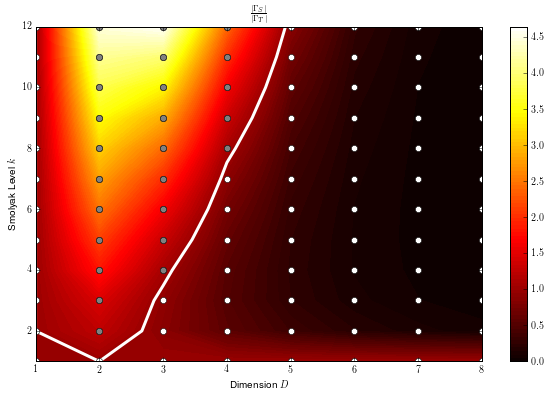
\includegraphics[width=0.8\linewidth]{./fig/smolyak_gauss_ratiomap.png}
  \end{figure}
\end{frame}

\begin{frame}{Smolyak construction issues}
  \begin{itemize}
    \item Solution:
    \begin{itemize}
      \item Search rules with nested nodes
      \item For interval $(-\infty, \infty)$ with weights $\exp(-x^2)$
      \item Iterative \emph{Kronrod} extensions
    \end{itemize}
  \end{itemize}
\end{frame}


\subsection{Kronrod Extension Schemes}

\begin{frame}{Kronrod Extensions}
  \begin{itemize}
    \item Goal: Find nested quadrature rules
    \item How?
  \end{itemize}
\end{frame}


\subsection{Genz-Keister Rules}


\begin{frame}{Smolyak construction}{Genz-Keister Nodes}
  \begin{figure}
    \centering
    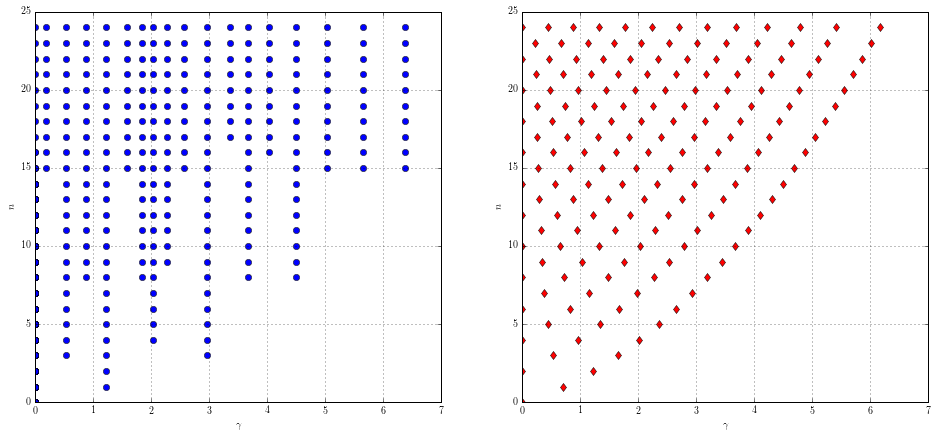
\includegraphics[width=\linewidth]{./fig/genz_keister_nodes.png}
  \end{figure}
\end{frame}

\begin{frame}{Smolyak construction}
  Construction with Genz-Keister nested rules
  \begin{figure}
    \centering
    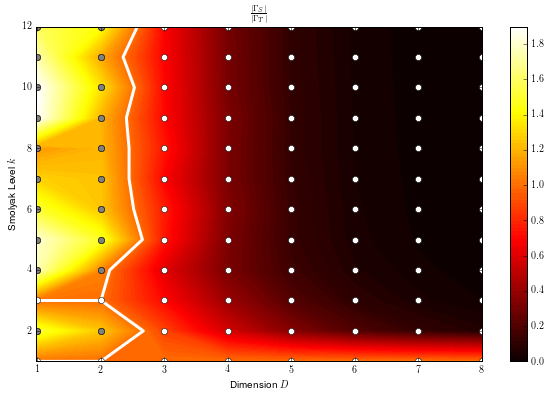
\includegraphics[width=0.8\linewidth]{./fig/smolyak_genzkeister_ratiomap.png}
  \end{figure}
\end{frame}


\begin{frame}{Final Solution for computing overlap Integrals}
  \begin{itemize}
    \item Chain of \emph{transformators}
    \begin{itemize}
      \item Steepest Descent: remove oscillations
      \item Sparse Grid: lessen curse of dimensionality
      \item Genz-Keister rules: nodes are nested
    \end{itemize}
  \end{itemize}
  \begin{figure}
    \centering
    \includegraphics[width=\linewidth]{./fig/diagram4.pdf}
  \end{figure}
\end{frame}



\section{Examples}

% Morse going wrong
% Harmonic Channel
% Harmonic Tube



\section{Future Work}

\begin{frame}
  \begin{itemize}
    \item Proof the steepest descent technique for unbounded intervals
    \item Other integrals like $\braket{\phi|V|\phi}$
    \item Potentials with exponential parts
    \item Proof for Kronrod Extensions
    \item Search for optimal rule
  \end{itemize}
\end{frame}


\section{End}

\begin{frame}{Thanks for your attention}
  \scriptsize
  \bibliographystyle{abbrv}
  \bibliography{mt}
\end{frame}

\end{document}
